\section{Experiments.}    
\paragraph{Models and Datasets.} 
To comprehensively evaluate the performance of SAES-SVD across diverse models and tasks, we conducted systematic experiments on mainstream open-source LLMs and standard language understanding and generation benchmarks, covering a wide range of parameter budgets and hardware settings. Unless otherwise specified, all results are obtained using a single-pass SVD per layer without task-specific fine-tuning after compression. For model selection, we considered representative architectures including LLaMA-1~\citep{touvron2023llama}, LLama-2~\citep{touvron2023llama2} and LLaMA-3~\citep{Meta2024Llama3}. Regarding evaluation tasks and datasets, we focused on natural language reasoning and understanding benchmarks. Specifically, we measured perplexity on the WikiText2~\citep{merity2016pointer} and C4~\citep{raffel2020exploring} dataset with a sequence length of 2048 to assess the language coherence and modeling capacity of the compressed models. In addition, we evaluated zero-shot accuracy on multiple datasets, including ARC-Challenge \citep{clark2018think}, ARC-Easy \citep{clark2018think}, HellaSwag \citep{zellers2019hellaswag}, MathQA~\citep{amini2019mathqa}, PIQA \citep{bisk2020piqa}, and WinoGrande \citep{sakaguchi2021winogrande}, to comprehensively examine the generalizability of the compressed models on various tasks.
\vspace{-0.3cm}
\paragraph{Baselines.}
In a unified calibration dataset and evaluation protocol, we compared our method with a range of well-established SVD-based low-rank compression approaches, including ASVD~\citep{li2025adasvd}, SVD-LLM~\citep{Wang2024SVD-LLM}, FW-SVD~\citep{Hsu2022FWSVD}, Dobi-SVD~\citep{wang2025dobi}, and AdaSVD~\citep{li2025adasvd}. Notably, SVD-LLM and Dobi-SVD rely on fine-tuning, while A-SVD, AdaSVD and Dobi-SVD employ mixed-rank strategies. In contrast, our proposed SAES-SVD does not require additional training nor auxiliary techniques, yet it consistently outperforms these baselines, highlighting its effectiveness and simplicity.

% ==== Requirements in preamble ====
% \usepackage{booktabs}
% \usepackage{multirow}
% \usepackage[table]{xcolor}
% \usepackage{graphicx} % for \resizebox

\begin{table*}[t]
\vspace{-1.2cm}
\centering
\small
\renewcommand{\arraystretch}{1.15}
\setlength{\tabcolsep}{2pt}
\newcommand{\na}{\textemdash}

\caption{Perplexity and zero-shot evaluation of LLaMA-7B across seven benchmark datasets under varying compression ratios. The table compares SAES-SVD with competing SVD-based methods (ASVD$^{*}$~\citep{yuan2023asvd}, FWSVD~\citep{Hsu2022FWSVD}, SVD-LLM$^{\dagger}$~\citep{Wang2024SVD-LLM}, Dobi-SVD$^{*\dagger}$~\citep{wang2025dobi}, Dip-SVD$^{*}$). Methods with fine-tuning are marked by $^{\dagger}$; mixed-rank strategies by $^{*}$. Due to the closed-source implementation of Dip-SVD, we were unable to obtain its performance at the 0.4 compression ratio.}
\resizebox{\textwidth}{!}{
\begin{tabular}{l l
                r r r | 
                c c c c c c
                c c c}
\toprule
\textbf{Ratio} & \textbf{Method} &
\textbf{Wiki2$\downarrow$} & \textbf{PTB$\downarrow$} & \textbf{C4$\downarrow$} &
\textbf{Openb.$\uparrow$} & \textbf{ARC\_e$\uparrow$} & \textbf{ARC\_c$\uparrow$} &
\textbf{WinoG.$\uparrow$} & \textbf{HellaS.$\uparrow$} & \textbf{PIQA$\uparrow$} &
\textbf{MathQA$\uparrow$} & \textbf{Avg.\,$\uparrow$} &
\textbf{Drop$\downarrow$} \\
\midrule
\multirow{1}{*}{\textbf{0.0}}
& Baseline & 5.68 & 8.35 & 7.34 & 0.28 & 0.67 & 0.38 & 0.67 & 0.56 & 0.78 & 0.27 & 0.52 & 0.00 \\
\midrule
\multirow{7}{*}{\textbf{0.2}}
& FWSVD         & 2e5 & 3e4   & 2e3  & 0.09  & 0.11  & 0.06  & 0.05  & 0.08  & 0.10  & 0.05  & 0.02 & 96\% \\
& ASVD$^\dagger$            & 11.14 & 16.55 & 15.93 & 0.25  & 0.53  & 0.27  & 0.64  & 0.41  & 0.68  & 0.24  & 0.43 & 16.7\% \\
& SVD-LLM$^\dagger$ & 7.94  & 16.22 & 15.84 & 0.22  & 0.58  & 0.29  & 0.63  & 0.43  & 0.69  & 0.24  & 0.44 & 14.7\% \\
& Dobi\mbox{-}SVD$^{*\dagger}$ & 8.54  & 14.83 & 10.01 & 0.26  & 0.59  & 0.31  & \textbf{0.66}  & 0.44  & 0.70  & 0.23  & 0.46 & 10.8\% \\
& Dip\mbox{-}SVD$^{*}$ & 7.95 & 15.60 & 14.07 & 0.27 & 0.63 & 0.33 & 0.64 & 0.45 & 0.71  & 0.24 & 0.47 & 9.2\% \\
\rowcolor{gray!12}
& \textbf{Ours}  & \textbf{7.17}  & \textbf{15.16}   & \textbf{13.77} & \textbf{0.29} & \textbf{0.68} & \textbf{0.36} & 0.65 & \textbf{0.45} & \textbf{0.75} & \textbf{0.25} & \textbf{0.50} & \textbf{3.9\%} \\
\midrule
\multirow{6}{*}{\textbf{0.4}}
& FWSVD         & 2e4 & 1e4 & 1e4 & 0.06  & 0.05  & 0.02  & 0.02  & 0.00  & 0.05  & 0.03  & 0.02 & 96.6\% \\
& ASVD$^\dagger$            & 1e3  & 3e3 & 1e3  & 0.13  & 0.28  & 0.22  & 0.48  & 0.26  & 0.55  & 0.19  & 0.30 & 41.8\% \\
& SVD-LLM$^\dagger$ & 13.11 & 63.75 & 49.83 & 0.19  & 0.42  & 0.25  & 0.58  & 0.33  & 0.60  & 0.21  & 0.37 & 28.3\% \\
& Dobi\mbox{-}SVD$^{*\dagger}$ & 13.54 & 46.38 & 23.54 & 0.22  & 0.41  & 0.27  & 0.58  & 0.34  & 0.61  & 0.23  & 0.38 & 26.3\% \\
& Dip\mbox{-}SVD$^{*}$  & 12.76 & 46.95 & 34.35 & 0.22 & 0.50 & \textbf{0.30} & 0.61 & 0.36 & 0.64  & 0.22 & 0.40 & 22.8\% \\
\rowcolor{gray!12}
& \textbf{Ours}  & \textbf{10.42} & \textbf{45.13}   & \textbf{32.79} & \textbf{0.23}   & \textbf{0.50}   & 0.29   & \textbf{0.62}   & \textbf{0.36}   & \textbf{0.65}   & \textbf{0.23 }  & \textbf{0.41} & \textbf{21.1\%} \\
\midrule
\multirow{5}{*}{\textbf{0.6}}
& FWSVD         & 3e4 & 2e4 & 2e4   & 0.06  & 0.01  & 0.00  & 0.00  & 0.01  & 0.01  & 0.00  & 0.01 & 97.8\% \\
& ASVD$^\dagger$            & 6e4 & 4e4 & 4e5 & 0.12  & 0.26  & 0.21  & 0.49  & 0.26  & 0.53  & 0.18  & 0.29 & 43.8\% \\
& SVD-LLM$^\dagger$ & 53.74 & 4e2 & 3e2 & 0.14  & 0.28  & 0.22  & 0.50  & 0.27  & 0.55  & 0.21  & 0.31 & 39.9\% \\
& Dobi\mbox{-}SVD$^{*\dagger}$ & 46.18 & 2e2 & 2e2 & 0.15  & 0.31  & 0.20  & 0.52  & 0.28  & 0.54  & 0.22  & 0.32 & 38.0\% \\
\rowcolor{gray!12}
& \textbf{Ours}  & \textbf{22.01} & \textbf{116.83} & \textbf{93.97} & \textbf{0.16}  & \textbf{0.33} & \textbf{0.25}  & \textbf{0.52} & \textbf{0.30} & \textbf{0.54} & \textbf{0.23} & \textbf{0.34} & \textbf{34.1\%} \\
\bottomrule
\end{tabular}
}
\label{tab main}
\end{table*}



\vspace{-0.3cm}
\paragraph{Main Results.}
We conducted a comprehensive evaluation of SAES-SVD for low-rank compression of LLMs and compared it with several SVD-based baselines across different compression ratios. Overall, SAES-SVD consistently achieved superior performance across tasks and model scales.
Table~\ref{tab main} summarizes results on the representative LLaMA-7B. SAES-SVD reduced the perplexity gap by more than 35\% compared with the strongest baseline and lowered the accuracy drop by 30–40\%. At the more challenging 0.6 ratio, it halved the perplexity gap relative to Dobi-SVD and SVD-LLM, while keeping the accuracy drop below 0.03, compared with more than 0.05 for other methods. 
These results lead to two key observations: (i) SAES-SVD consistently reduces perplexity by a large margin—up to a 2$\times$ improvement at aggressive compression levels—and (ii) it preserves or even improves accuracy, while other methods suffer notable degradation. Crucially, SAES-SVD outperforms not only methods requiring fine-tuning (e.g., SVD-LLM, Dobi-SVD) but also those relying on mixed-rank allocations (e.g., AdaSVD, Dobi-SVD,Dip-SVD). 
% Together with the additional experiments presented in the appendix and subsequent tables, 
These findings, together with additional experiments shown in Table~\ref{tab:27b} and Table~\ref{tab:38b} in appendix,  confirm that the gains of SAES-SVD generalize across architectures and model scales, underscoring both its robustness and broad applicability. 


\begin{table}[t]
\centering
\small
\renewcommand{\arraystretch}{1.15}
\setlength{\tabcolsep}{5pt}
\newcommand{\na}{\textemdash}
\caption{
Zero-shot accuracy of LLaMA-13B under different compression ratios on seven benchmark datasets. Results are reported for SVD-LLM$^{\dagger}$, Dip-SVD$^{*}$, and our proposed method. $^{\dagger}$ denotes methods that rely on fine-tuning, while $^{*}$ indicates methods using mixed-rank strategies.
}
\begin{tabular}{l l| c c c c c c c | c}
\toprule
\textbf{Ratio} & \textbf{Method} &
\textbf{Openb.} & \textbf{ARC\_e} & \textbf{WinoG.} & \textbf{HellaS.} &
\textbf{ARC\_c} & \textbf{PIQA} & \textbf{MathQA} & \textbf{Average} \\
\midrule
\multirow{3}{*}{\textbf{0.2}}
& SVD-LLM$^\dagger$  & 0.302 & 0.683 & 0.684 & 0.470 & 0.356 & 0.725 & 0.265 & 0.498 \\
& Dip-SVD$^*$  & 0.306 & 0.681 & \textbf{0.692} & \textbf{0.490} & 0.369 & 0.734 & 0.258 & 0.504 \\
\rowcolor{gray!12}
& \textbf{Ours} & \textbf{0.308} & \textbf{0.712} & 0.684 & 0.477 & \textbf{0.388} & \textbf{0.734} & \textbf{0.265} & \textbf{0.510} \\
\midrule
    \multirow{3}{*}{\textbf{0.4}}
& SVD-LLM$^\dagger$  & 0.222 & 0.521 & 0.639 & 0.355 & 0.248 & 0.637 & 0.228 & 0.407 \\
& Dip-SVD$^*$  & 0.230 & 0.548 & 0.644 & 0.402 & 0.283 & \textbf{0.661} & 0.233 & 0.429 \\
\rowcolor{gray!12}
& \textbf{Ours} & \textbf{0.248} & \textbf{0.543} & \textbf{0.654} & \textbf{0.470} & \textbf{0.284} & 0.631 & \textbf{0.239} & \textbf{0.438} \\
\bottomrule
\end{tabular}
\vspace{-0.5cm}
\label{tab large models}
\end{table}



% \begin{table}[t]
% \centering
% \small
% \renewcommand{\arraystretch}{1.15}
% \setlength{\tabcolsep}{5pt}
% \newcommand{\na}{\textemdash}

% \begin{tabular}{l l c c c c c c c c}
% \toprule
% \textbf{Ratio} & \textbf{Method} &
% \textbf{Openb.} & \textbf{ARC\_e} & \textbf{WinoG.} & \textbf{HellaS.} &
% \textbf{ARC\_c} & \textbf{PIQA} & \textbf{MathQA} & \textbf{Average} \\
% \midrule
% \multirow{5}{*}{\textbf{0.8}}
% & ASVD$^\dagger$     & 0.330 & 0.732 & 0.707 & 0.540 & 0.431 & 0.771 & 0.251 & 0.538 \\
% & FWSVD    & 0.312 & 0.737 & 0.696 & 0.518 & 0.393 & 0.769 & 0.258 & 0.526 \\
% & SVD-LLM$^\dagger$  & 0.302 & 0.683 & 0.684 & 0.470 & 0.356 & 0.725 & 0.265 & 0.498 \\
% & Dip-SVD$^*$  & 0.306 & 0.681 & 0.692 & 0.490 & 0.369 & 0.734 & 0.258 & 0.504 \\
% \rowcolor{gray!12}
% & \textbf{Ours} & 0.308 & 0.712 & 0.684 & 0.477 & 0.388 & 0.734 & 0.265 & 0.510 \\
% \midrule
% \multirow{5}{*}{\textbf{0.6}}
% & ASVD$^\dagger$     & 0.148 & 0.336 & 0.518 & 0.293 & 0.197 & 0.579 & 0.215 & 0.327 \\
% & FWSVD    & 0.166 & 0.431 & 0.552 & 0.305 & 0.219 & 0.607 & 0.226 & 0.358 \\
% & SVD-LLM$^\dagger$  & 0.222 & 0.521 & 0.639 & 0.355 & 0.248 & 0.637 & 0.228 & 0.407 \\
% & Dip-SVD$^*$  & 0.230 & 0.548 & 0.644 & 0.402 & 0.283 & 0.661 & 0.233 & 0.429 \\
% \rowcolor{gray!12}
% & \textbf{Ours} & 0.248 & 0.543 & 0.654 & 0.470 & 0.284 & 0.631 & 0.239 & 0.438 \\
% \bottomrule
% \end{tabular}
% \caption{
% Zero-shot accuracy of LLaMA-13B under different compression ratios on seven benchmark datasets. Results are reported for ASVD, FWSVD, SVD-LLM$^{\dagger}$, Dip-SVD$^{}$, and our proposed method. $^{\dagger}$ denotes methods that rely on fine-tuning, while $^{*}$ indicates mixed-rank variants. 
% % Our approach consistently outperforms or matches prior methods across both compression settings (0.8 and 0.6), achieving higher average accuracy without fine-tuning or mixed-rank techniques.
% }
% \label{tab large models}
% \end{table}
\vspace{-0.3cm}
\paragraph{Comparison on larger-scale models.} We further evaluated our method on larger architectures, including LLaMA-13B and LLaMA-30B, against current SOTA approaches. As shown in Table~\ref{tab large models} and Figure~\ref{fig llama_30b ppl}, we conducted experiments across compression ratios ranging from 0.2 to 0.4. Our method consistently outperforms all baselines in terms of both average accuracy and perplexity. Notably, on LLaMA-30B, SAES-SVD reduces perplexity to 5.49, compared with 22.71 for ASVD and 5.63 for SVD-LLM( Note that Dip-SVD results are only available for 7B and 13B, since the original work does not report LLaMA-30B and its implementation is not publicly released), while achieving a 10\% accuracy improvement over Dip-SVD. These results demonstrate that SAES-SVD remains highly effective at larger scales and delivers substantial gains in compressed model performance.
\vspace{-0.3cm}
\begin{figure}[t]
    \vspace{-1.2cm}
    \centering
    % 第一张图
    \begin{minipage}[t]{0.49\textwidth}
        \centering
        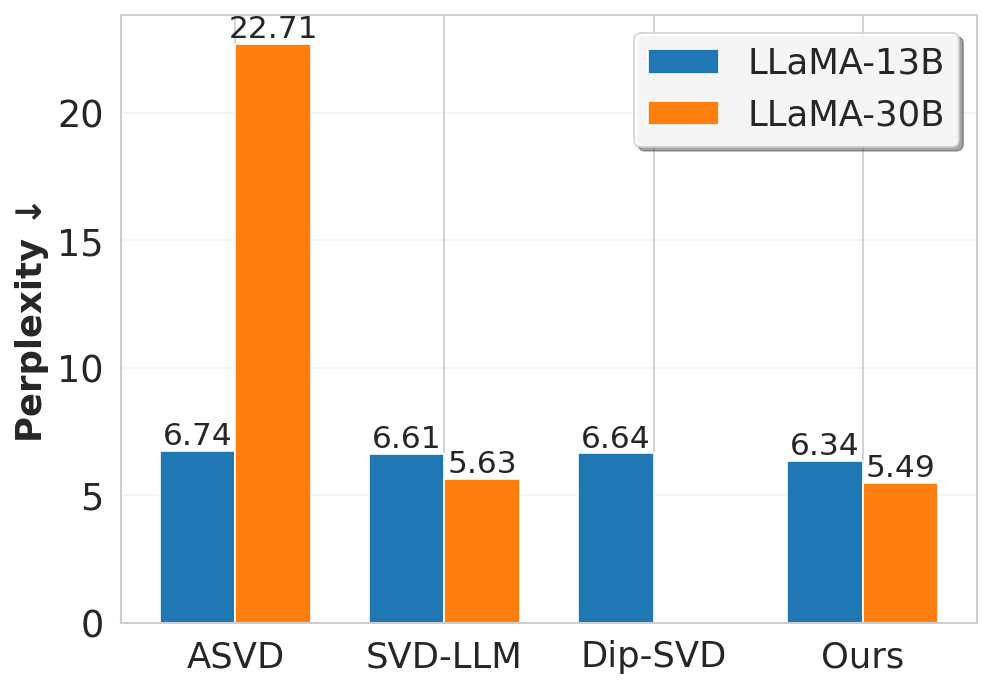
\includegraphics[width=\linewidth, trim= 5 5 5 5, clip]{figs/llama13b_30b_ppl.png}
        \caption{Wiki-PPL for two large-scale models, across different methods at 20\% compression.}
        \label{fig llama_30b ppl}
    \end{minipage}
    \hfill
    % 第二张图
    \begin{minipage}[t]{0.49\textwidth}
        \centering
        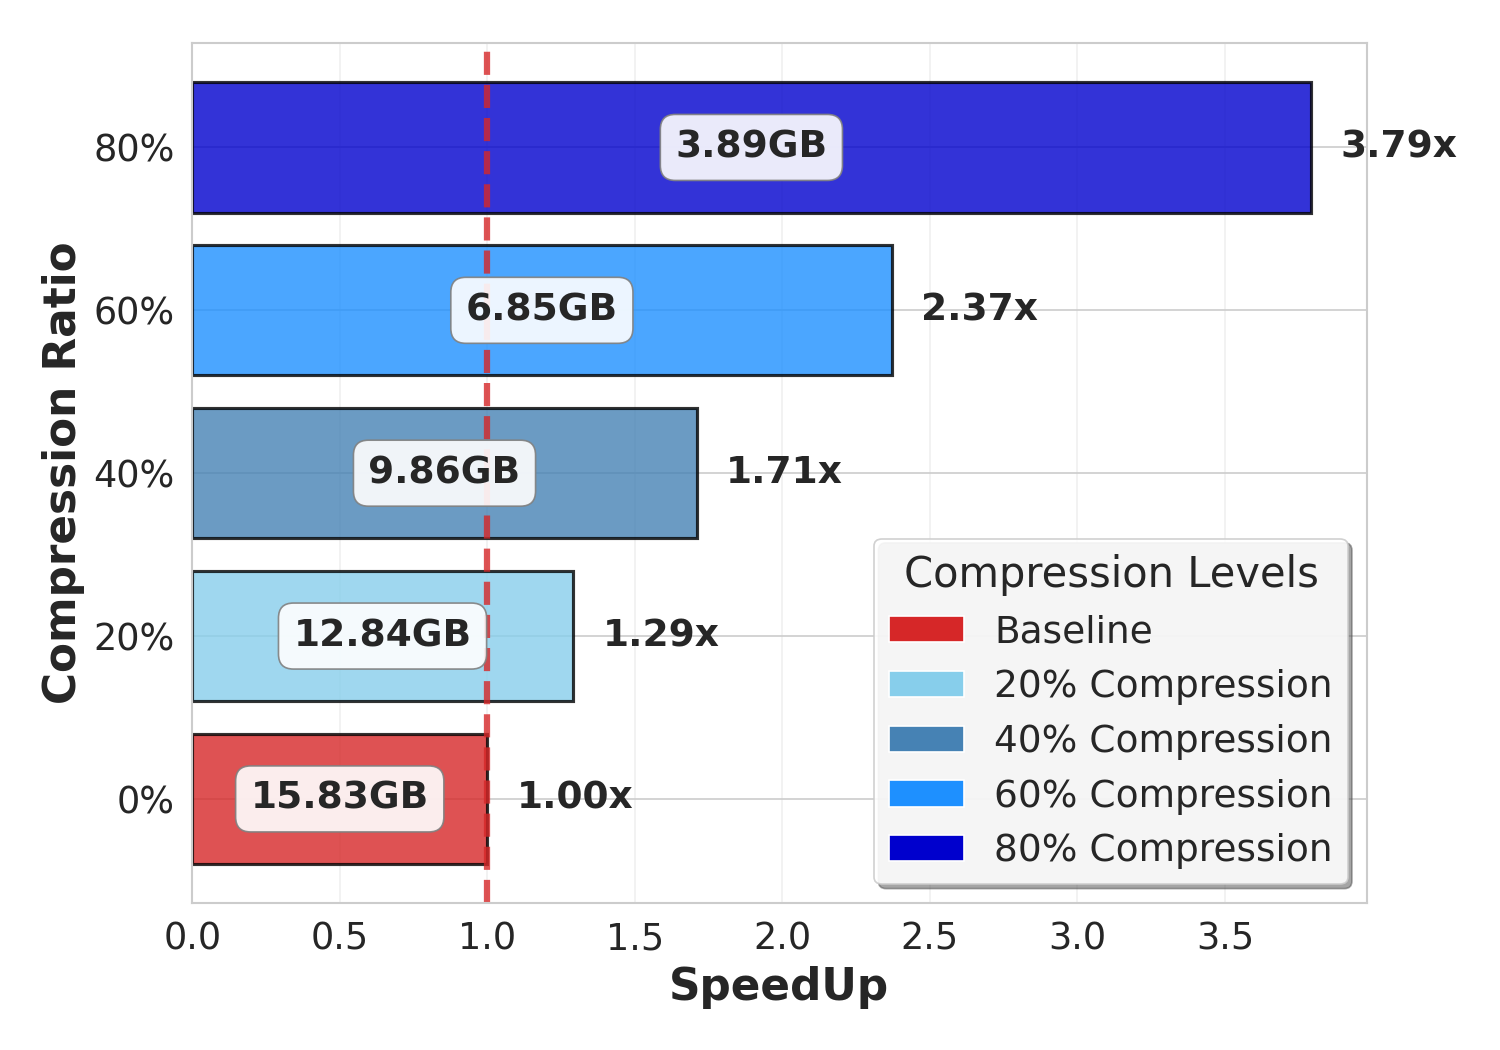
\includegraphics[width=\linewidth, trim=20 10 20 10, clip]{figs/speed_up_memory_usage.png}
        \caption{Memory usage and inference speedup of LLaMA-3-8B on varying compression ratios.}
        \label{fig speedup}
    \end{minipage}
    \vspace{-0.2cm}
\end{figure}

\vspace{-2mm}
\paragraph{Inference speed.} Low-rank approximation simultaneously decreases both computational complexity and parameter storage. This dual reduction substantially lowers memory footprint and compute requirements. We evaluated the inference speed of LLaMA3-8B under different compression ratios on a single NVIDIA A6000 GPU. As illustrated in Figure~\ref{fig speedup}, our proposed SAES-SVD achieves consistent acceleration over the FP16 baseline, with speedups ranging from 1.29× to 3.79× as the compression ratio increases. These results demonstrate the practicality of SAES-SVD in accelerating inference while significantly reducing memory demands.


\vspace{-0.3cm}
\paragraph{Ablation Experiments.}   

The proposed SAES-SVD framework consists of two complementary components: Cumulative Error-Aware Layer Compression (CEALC) and Adaptive Collaborative Error Suppression (ACES). CEALC addresses the limitation of prior methods that treat layer compression as independent processes; as shown in Figure~\ref{fig:sub1}, it effectively mitigates cumulative compression errors. Building on this, ACES further enhances the low-rank properties of the compression objective shaped by CEALC, leading to superior performance under limited rank budgets, as illustrated in Figure~\ref{fig different alpha}. The ablation results presented in Table~\ref{table ablation 1} confirm these contributions: CEALC significantly improves both generative and zero-shot tasks, while ACES provides additional performance gains on top of CEALC.
\begin{table}[t]
\centering
\begin{minipage}[t]{0.45\textwidth}
    \centering
    \small
    \renewcommand{\arraystretch}{1.15}
    \setlength{\tabcolsep}{5pt}
    \caption{Ablation study on the two components of our method. Avg Acc denotes the average accuracy over PIQA, ARC-e, HellaSwag and WinoGrande.}
    \begin{tabular}{l c c c c}
    \toprule
    \textbf{Model} & CEALC & ACES & \textbf{Wiki PPL$\downarrow$} & \textbf{Avg Acc$\uparrow$} \\
    \midrule
    LLama2-7B & $\times$ & $\times$ & 9.34  & 58.66 \\
              & $\checkmark$ & $\times$ & 7.66  & 62.02 \\
              & $\checkmark$ & $\checkmark$ & 7.37  & 63.03 \\
    \midrule
    LLama3-8B & $\times$ & $\times$ & 16.59 & 55.76 \\
              & $\checkmark$ & $\times$ & 12.25 & 58.82 \\
              & $\checkmark$ & $\checkmark$ & 11.48 & 60.18 \\
    \bottomrule
    \end{tabular}
    \label{table ablation 1}
\end{minipage}\hfill
\begin{minipage}[t]{0.45\textwidth}
    \centering
    \small
    \renewcommand{\arraystretch}{1.15}
    \setlength{\tabcolsep}{5pt}
    \caption{Sensitivity analysis of the upper and lower bounds of the adaptive coefficient $\alpha$ in ACES, conducted on LLaMA2-7B at a 20\% compression ratio.}
    \begin{tabular}{c c c c}
    \toprule
    $\alpha_{\min}$ & $\alpha_{\max}$ & \textbf{Wiki PPL$\downarrow$} & \textbf{Avg Acc$\uparrow$} \\
    \midrule
    0   & 1   & 8.96 & 58.47 \\
    0.1 & 0.9 & 7.88 & 62.81 \\
    0.2 & 0.8 & 7.38 & 63.02 \\
    0.25& 0.75& 7.37 & 63.03 \\
    0.3 & 0.7 & 7.36 & 63.01 \\
    0.4 & 0.6 & 7.63 & 62.87 \\
    \bottomrule
    \end{tabular}
    \label{tab ablation 2}
    \label{tab ablation alpha}
\end{minipage}
\vspace{-0.5cm}
\end{table}


We conducted a sensitivity analysis of the adaptive coefficient $\alpha$ by varying its lower and upper bounds. Experiments were performed on LLaMA-2 7B at a 20\% compression ratio, with results summarized in Table~\ref{tab ablation 2}. The analysis shows that performance is relatively stable within moderate ranges of $\alpha$. Specifically, when $\alpha_{\min}=0.25$ and $\alpha_{\max}=0.75$, the model achieves the best trade-off, with an average zero-shot accuracy of 63.03\%. In contrast, setting the lower bound too high (e.g., $\alpha_{\min} > 0.8$) slightly degrades perplexity while reducing average accuracy significantly, indicating potential overfitting calibration dataset. These results validate our choice of setting the lower bound to 0.25 and the upper bound to 0.75 in practice.


